\documentclass[12pt]{article}
%Gummi|065|=)
\usepackage{amsmath, amsfonts, amssymb}
\usepackage[margin=0.5in]{geometry}
\usepackage{xcolor}
\usepackage{graphicx}

\newcommand{\off}[1]{}
\DeclareMathSizes{20}{30}{20}{18}

\newcommand{\two }{\sqrt[3]{2}}
\newcommand{\four}{\sqrt[3]{4}}
\newcommand{\red}{\begin{tikz}[scale=0.25]
\draw[fill=red, color=red] (0,0)--(1,0)--(1,1)--(0,1)--cycle;\end{tikz}}
\newcommand{\blue}{\begin{tikz}[scale=0.25]
\draw[fill=blue, color=blue] (0,0)--(1,0)--(1,1)--(0,1)--cycle;\end{tikz}}
\newcommand{\green}{\begin{tikz}[scale=0.25]
\draw[fill=green, color=green] (0,0)--(1,0)--(1,1)--(0,1)--cycle;\end{tikz}}

\usepackage{tikz}

\title{Curve Fitting}
\author{John D Mangual}
\date{}
\begin{document}

\fontfamily{qag}\selectfont \fontsize{12.5}{15}\selectfont

\maketitle

\noindent I feel there are ways to do curve-fitting that look up and down the ladder of abstractions.  Let's start with something pretty vanilla: \\ \\
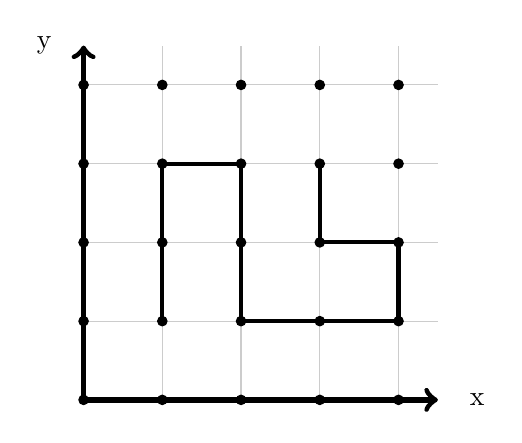
\begin{tikzpicture}

\node at ( 5,0) {x};
\node at (-0.5,4.5) {y};

\foreach \a in {0,...,4}{ 
	\draw[color=black!20!white] (\a,0)--(\a,4.5);
	\draw[color=black!20!white] (0,\a)--(4.5,\a);
 }

\draw[line width=2, ->] (0,0)--(4.5,0);
\draw[line width=2, ->] (0,0)--(0,4.5);

\foreach \a in {0,...,4}{
\foreach \x in {0,...,4}{
			\draw[fill=black] (\a,\x) circle (0.06);
	 }
}


\draw[line width=1.5] (1,1)--(1,2)--(1,3)--(2,3)--(2,1)--(4,1)--(4,2)--(3,2)--(3,3);
\end{tikzpicture} \\ 
Can we draw a curve that passes through all these points?  There are two strategies to try to hook around this many constraints:
\begin{itemize}
\item Lagrange Interpolation
\item Bezier Curves
\end{itemize} 
And maybe it depends on the type of constraint problem you are trying to solve: 
\begin{itemize}
\item passing through points
\item weaving arround points
\end{itemize}
I think one way to motivate a theory is to start with a problem you want to solve.\footnote{Other times, theories comes out of the box, complete. I think such theories are unusuable, or they leave from for input from you and me.  A comeback from that camp could be, ``John, why are you so obsessed with this particular problem?"  And I don't have any good reason.  Just because.  Sometimes about me, and the time and place makes me interested.  And I could be wrong!} We like to brag about how good we are at weaving around constraints.  How bad can we be?  Let $f: [0,1] \to \mathbb{R}$ be a real-valued function:
$$ f(x) = \left\{  \begin{array}{cc} 1 & x \notin \mathbb{Q}  \\ 
0 & x \in \mathbb{Q} \end{array} \right. $$
Then we can ask what the integral is between $0$ and $1$.  Overwhelmingly, the answer should be:
$$ \int_0^1 f(x) \, dx = 1 \times \Big|\{ x \notin \mathbb{Q}  \}\cap [0,1]\Big| + 0 \times \Big|\{ x \in \mathbb{Q}  \}\cap [0,1]\Big| =  1 $$
Relatively innocent-functions like these are sufficient Riemann integration.  I reasoned there are vastly more irrational numbers than rational numbers.


\newpage

\noindent This turns out to be one of the worse functions around, because it looks like $\mathbf{1}$ but isn't:
$$ f(x) \approx \mathbf{1} \quad\text{therefore}\quad \int f \approx \int \mathbf{1} $$
If I recall, we placed intervals around every single fraction $\frac{a}{b} \in \mathbb{Q}$ we get an upper estimate for how large this integral could be, and that upper estimate $ \to 0$.   \\ \\
How to deal with a function that often looks like $f(x) \equiv 1$ but isn't?\footnote{
One set of problems that plagued me was if we had two competing definition of  limit, maybe one returns a number and the other does not.  If we have two limiting procedures $1$ and $2$, maybe: 
$$ \big[ \lim \big]_1 \; a_n = A \quad\text{implies}\quad \big[ \lim \big]_2 \; a_n = A$$
Most of the time we don't really care how the limit procedure is defined.  Who cares really?
$$ N \gg 1 \quad \text{implies}\quad a_N \approx A$$
and the impliciation looks self-evident and most people won't question it.  The only reason we remember the exception is because that particular conversation went on record.} \\ 
\includegraphics{farey-01.png} \\
Here is a plot if we add all of the pure tones at all frequencies $\frac{a}{b}$ with $0 < a < b < 10$.  Theoretically we have found:
$$ \frac{1}{28} \sum_{0 < a < b < 10} e^{2\pi i \frac{a}{b} t} \approx \frac{1}{ c\, N^2 }  \sum_{0 < a < b < N} e^{2\pi i \frac{a}{b} t}
= \left\{ \begin{array}{cc}  1 & \text{if }t = 0 \\ 0 & \text{if }t \neq 0\end{array} \right.  $$
The constant in front is an oversimplification.  The odds of two numbers being relatively primes is a famous one:
$$ \phi(1) + \phi(2) + \dots + \phi(N) = \# \{ (a,b) : a < b \text{ and } \mathrm{gcd}(a,b)=1 \} \approx \frac{2}{\zeta(2)^2} $$
Analysis is the branch of math where we account for all the uses of the $\approx$  symbol.  What if I told you the function we just charted is $\approx {\color{blue}\mathbf{0}}$ ?

\newpage

\noindent When I read someone else's paper, a lot of my surprise stems from the author suggesting there is enough from in function space for something (very unlikely) to occur.  Let's make a little problem set: \\ \\
\# \textbf{1} Show constant function on the rational numbers integrates to zero:
$$ \int_{[0,1]} \mathbf{1}_{\mathbb{Q}} = 0 $$ 
\# \textbf{2} Find a curve that weaves around the obstacle course on page one:\\ \\
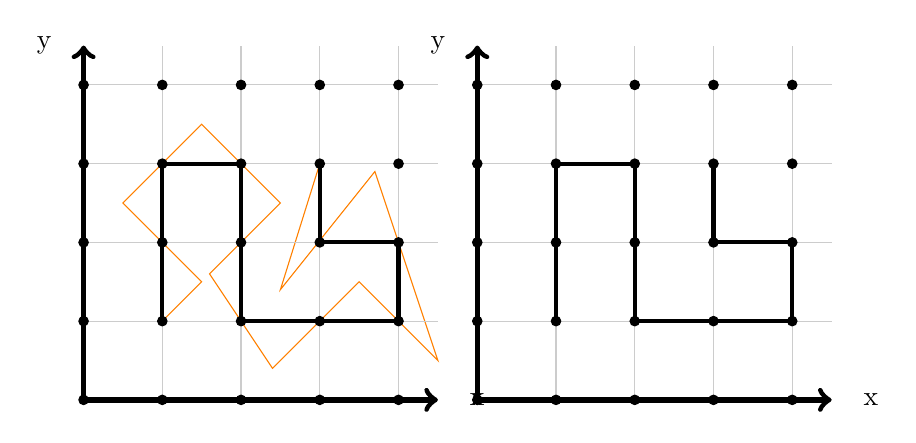
\begin{tikzpicture}

\begin{scope}

\node at ( 5,0) {x};
\node at (-0.5,4.5) {y};

\draw[color=red!50!yellow] (1, 1)--(1.5,1.5)--(0.5,2.5)--(1.5,3.5)--(2.5,2.5)--(1.6,1.6)--(2.4,0.4)
--(3.5,1.5)--(4.5,0.5)--(3.7,2.9)--(2.5,1.4)--(3,3);

\foreach \a in {0,...,4}{ 
	\draw[color=black!20!white] (\a,0)--(\a,4.5);
	\draw[color=black!20!white] (0,\a)--(4.5,\a);
 }

\draw[line width=2, ->] (0,0)--(4.5,0);
\draw[line width=2, ->] (0,0)--(0,4.5);

\foreach \a in {0,...,4}{
\foreach \x in {0,...,4}{
			\draw[fill=black] (\a,\x) circle (0.06);
	 }
}


\draw[line width=1.5] (1,1)--(1,2)--(1,3)--(2,3)--(2,1)--(4,1)--(4,2)--(3,2)--(3,3);



\end{scope}

\begin{scope}[xshift=5cm]

\node at ( 5,0) {x};
\node at (-0.5,4.5) {y};

\foreach \a in {0,...,4}{ 
	\draw[color=black!20!white] (\a,0)--(\a,4.5);
	\draw[color=black!20!white] (0,\a)--(4.5,\a);
 }

\draw[line width=2, ->] (0,0)--(4.5,0);
\draw[line width=2, ->] (0,0)--(0,4.5);

\foreach \a in {0,...,4}{
\foreach \x in {0,...,4}{
			\draw[fill=black] (\a,\x) circle (0.06);
	 }
}


\draw[line width=1.5] (1,1)--(1,2)--(1,3)--(2,3)--(2,1)--(4,1)--(4,2)--(3,2)--(3,3);

\end{scope}

\end{tikzpicture} 
With a pencil it's always possible to draw a curve that passes through all the dots.
Our challenge is to find an equation that passes through all the loops.  This is not so obvious it can always be done. \\ \\
\# \textbf{3} While I am remembering that my other example was going to be, we are going to solve the Prime Number Theorem.  
$$ \Lambda(n) = \left\{ \begin{array}{cl} \log p & \text{if }n=p \\ \\
0 & \text{not prime}\end{array} \right. $$
The prime number says that the density of primes is roughly $ \frac{1}{\text{\# digits}} $ it can also be phrased as:
$$ \sum_{n \leq x} \Lambda(n)  = x + o(x) $$
where $o(x)$ is a really small, unpredictible number\footnote{if you looked at my other projects, a great question to ask would be ``how small", and ``how unpredictible".  We could ask even though $o(x)$ is a small number, maybe it is bigger than $1$ or $5$ or $100$.} This won't be a review of number theory.  Just ironing out one or two parts in a previous discussion.  It's pretty hard. \\ \\
\# \textbf{4} Look at a real paper.  There are one or two short papers of Bourgain that I try to get through from time to time.\footnote{He does not write in a very forgiving way, and occasionally it's so bad, we may as well try to write the step ourselves.}
$$ f(t) = \sum_{|x|, |y|, |z| < N} e^{2\pi i t \; (x^2 + y^2 - \sqrt{2} z^2)} $$ 
This is my favorite way to cause trouble and I get the sense this is the recommended way to start.  A sense that comes from nowhere. .
 \\ \\

\newpage

\vfill


\noindent 

\begin{thebibliography}{}

\item \dots 


\end{thebibliography}

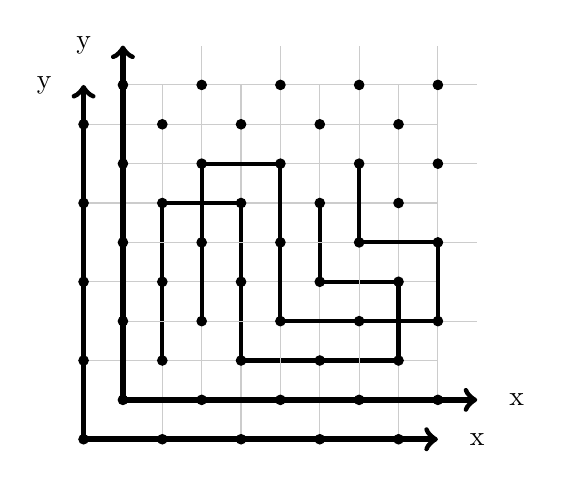
\begin{tikzpicture}

\node at ( 5,0) {x};
\node at (-0.5,4.5) {y};

\foreach \a in {0,...,4}{ 
	\draw[color=black!20!white] (\a,0)--(\a,4.5);
	\draw[color=black!20!white] (0,\a)--(4.5,\a);
 }

\draw[line width=2, ->] (0,0)--(4.5,0);
\draw[line width=2, ->] (0,0)--(0,4.5);

\foreach \a in {0,...,4}{
\foreach \x in {0,...,4}{
			\draw[fill=black] (\a,\x) circle (0.06);
	 }
}


\draw[line width=1.5] (1,1)--(1,2)--(1,3)--(2,3)--(2,1)--(4,1)--(4,2)--(3,2)--(3,3);


\begin{scope}[xshift=0.5cm, yshift=0.5cm]

\node at ( 5,0) {x};
\node at (-0.5,4.5) {y};

\foreach \a in {0,...,4}{ 
	\draw[color=black!20!white] (\a,0)--(\a,4.5);
	\draw[color=black!20!white] (0,\a)--(4.5,\a);
 }

\draw[line width=2, ->] (0,0)--(4.5,0);
\draw[line width=2, ->] (0,0)--(0,4.5);

\foreach \a in {0,...,4}{
\foreach \x in {0,...,4}{
			\draw[fill=black] (\a,\x) circle (0.06);
	 }
}


\draw[line width=1.5] (1,1)--(1,2)--(1,3)--(2,3)--(2,1)--(4,1)--(4,2)--(3,2)--(3,3);
\end{scope}


\end{tikzpicture}



\end{document}